\documentclass[11pt,slides,aspectratio=43]{beamer}
\usepackage[utf8]{inputenc}
\usepackage[russian]{babel}
\usepackage{xcolor}
\usepackage{multicol}
\usepackage{ragged2e}

\usepackage{amsmath}
\usepackage{amsfonts}
\usepackage{amssymb}
\usepackage{amsthm}


\usetheme{Warsaw} %Dresden %Warsaw
\usecolortheme{whale} %wolverine
%\beamertemplatetransparentcovereddynamicmedium
\beamertemplateshadingbackground{yellow!20}{yellow!50}
%\beamertemplategridbackground[15]

\title[]{Шахматоподобные игры}
\author[Ежков М. Поляков Д.]{Ежков Марк \\Поляков Денис}
\date{23 мая 2014 г.}

\begin{document}

	\begin{frame}
		\maketitle
	\end{frame}
	\section{Постановка задачи}	
	\begin{frame}
	\frametitle{Основные идеи и принципы}
	   \begin{block}{}
            \begin{itemize}
	           \item Возможность играть в произвольные шахматоподобные игры в одном приложения.
	           \item Правила игры описываются на XML.
               \item Приложение должно обладать графическим интерфейсом и искусственным интеллектом.
            \end{itemize}
		\end{block}
	\end{frame}
	
	\section{Описание языка}%
	\begin{frame}{Параметры игрового поля. Начальная расстановка.}
		\begin{block}{}
            \begin{itemize}
	           \item Наиболее простой и естественной частью языка является описание игрового поля и начальной расстановки фигур.
            \end{itemize}
            \begin{center}
			     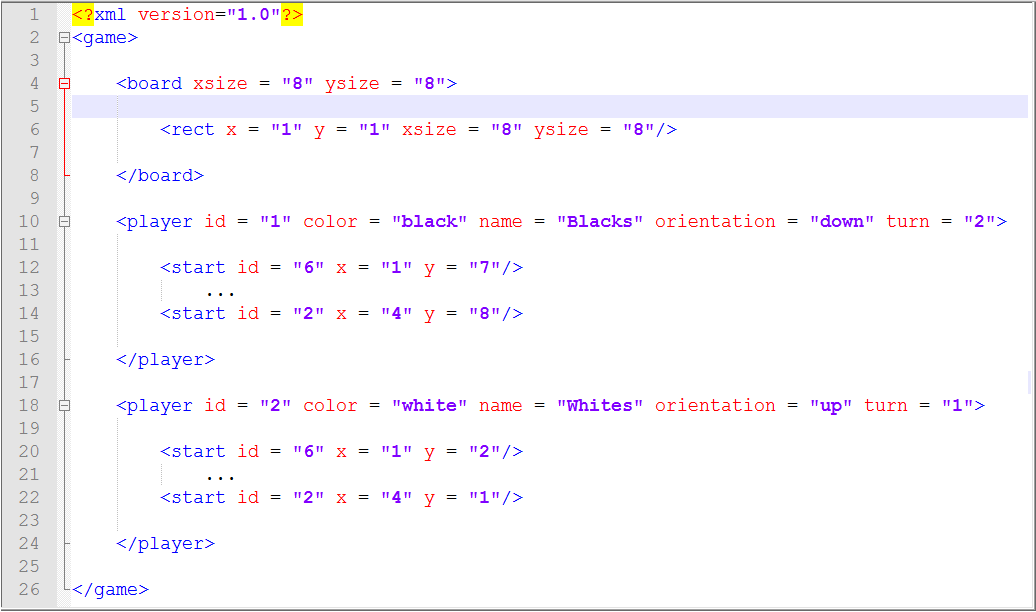
\includegraphics[scale=0.33]{gameBoard.png}
		    \end{center}
		\end{block}
	\end{frame}

    \begin{frame}{Описание игровых фигур.}
		\begin{block}{}
            \begin{itemize}
	           \item Фигура обладает набором атрибутов: id, weight, image.
            \end{itemize}
            \begin{center}
			     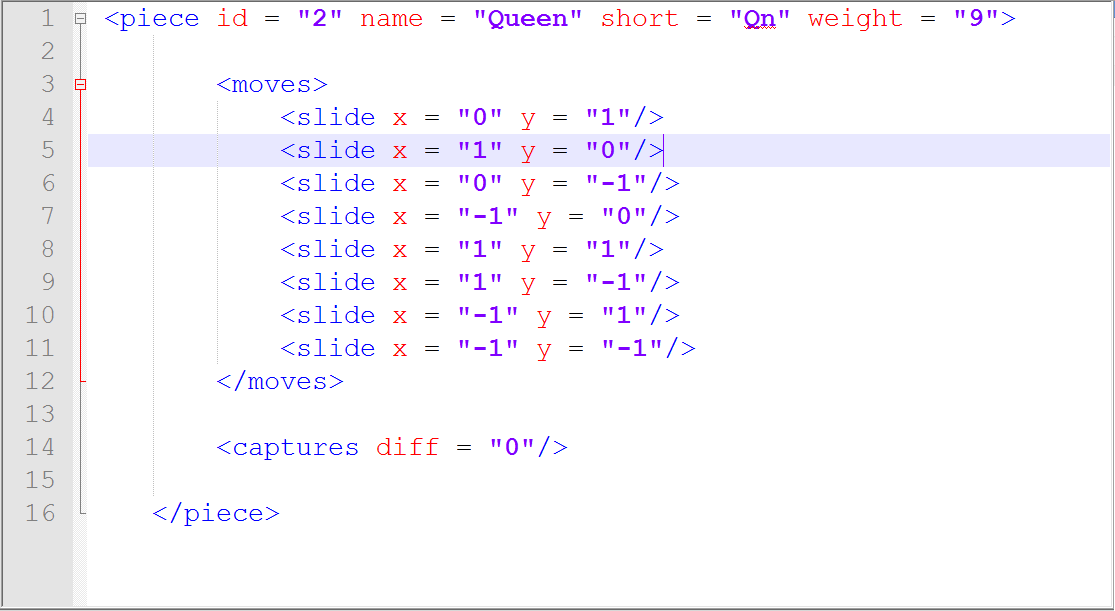
\includegraphics[scale=0.33]{attributes.png}
		    \end{center}
		\end{block}
	\end{frame}

    \begin{frame}{Описание игровых фигур.}
		\begin{block}{}
            \begin{itemize}
	           \item Простые перемещения и взятия описываются тегами <jump/> и <slide/>.
            \end{itemize}
            \begin{center}
			     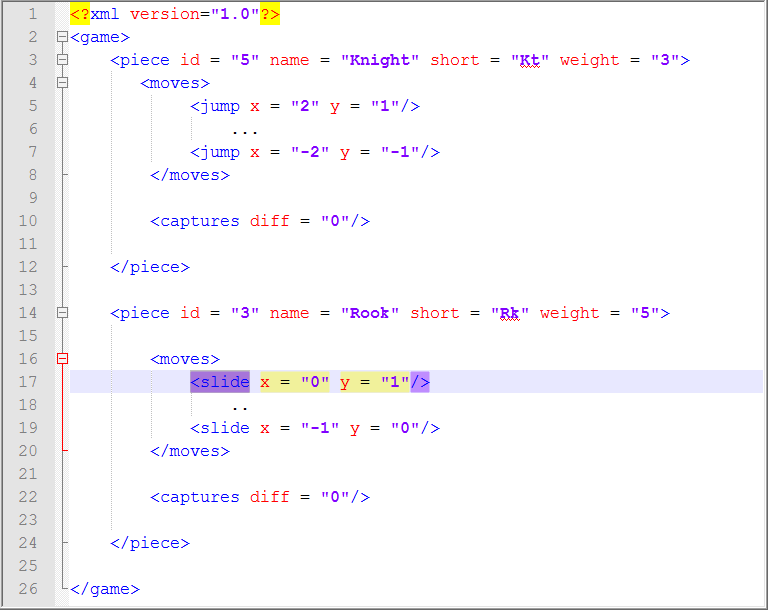
\includegraphics[scale=0.33]{pieces.png}
		    \end{center}
		\end{block}
	\end{frame}

    \begin{frame}{Описание игровых фигур.}
		\begin{block}{}
            \begin{itemize}
	           \item Сложные ходы, например взятие на проходе, описываются тегом <special/>.
            \end{itemize}
            \begin{center}
			     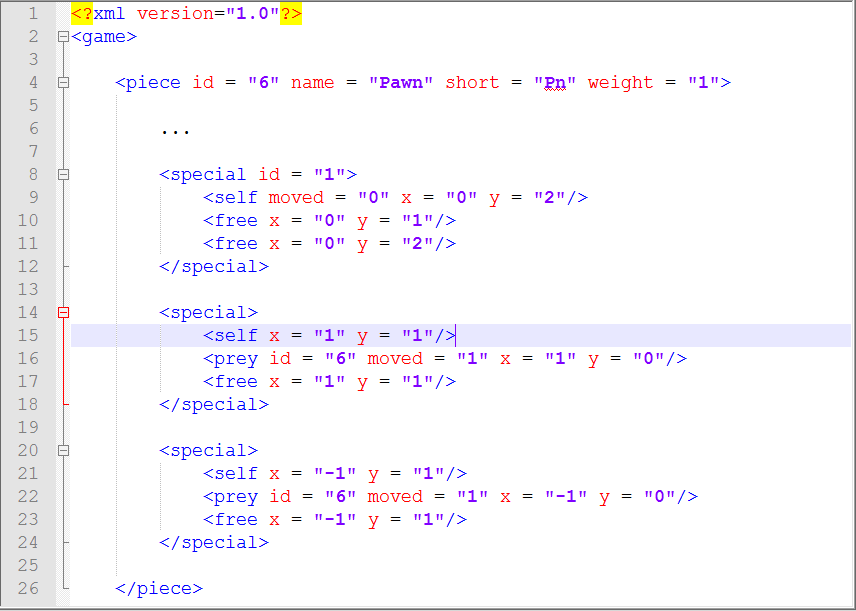
\includegraphics[scale=0.33]{special.png}
		    \end{center}
		\end{block}
	\end{frame}

    \section{Описание модели. Тесты}

     \begin{frame}{Модель}
	
	\end{frame}

    \begin{frame}{Тесты}
		\begin{itemize}
	           \item Для тестирования мы использовали unit testing.
               \item Главной задачей тестирования была проверка корректности выполнения ходов.
               \item Модель позволяет в теле теста автоматически разыгрывать различные шахматные партии и их части.
        \end{itemize}
	\end{frame}

    \section{Искусственный интеллект}

    \begin{frame}{Искусственный интеллект.}
		\begin{itemize}
	           \item Интеллект реализуется алгоритмом минимакса с модификацией: альфа-бета отсечение.
        \end{itemize}
        \begin{center}
			     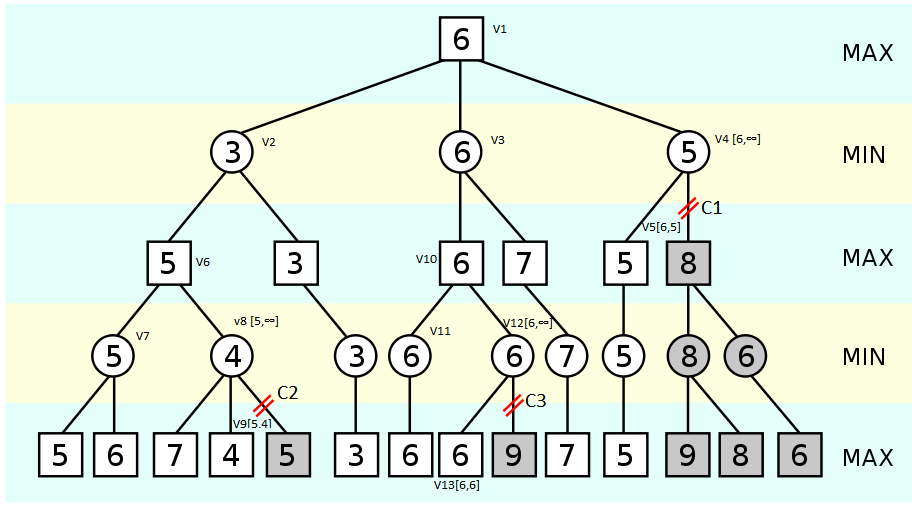
\includegraphics[scale=0.33]{tree.png}
		\end{center}
	\end{frame}

    \begin{frame}{Искусственный интеллект.}
		\begin{itemize}
               \item Для работы интеллекта требуется оценочная функция позиции и список всех возможных ходов, также необходимо создавать копии объекта Game.
        \end{itemize}
        \begin{center}
			     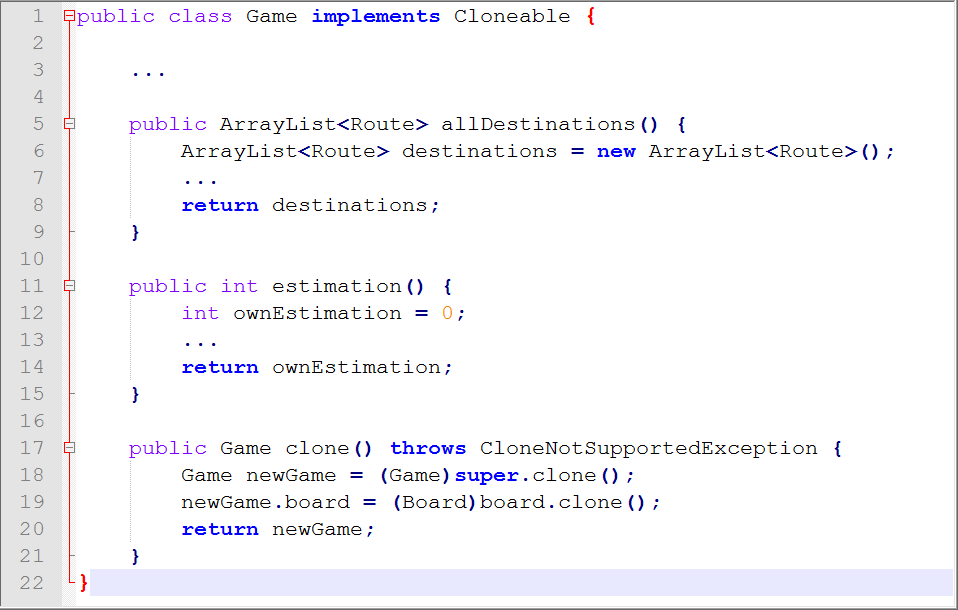
\includegraphics[scale=0.33]{gameAI.png}
		\end{center}
	\end{frame}
	
\end{document} 